%! Author = drakanoy
%! Date = 10.09.2024

% Preamble
\documentclass[12pt]{article}

% Packages
\usepackage[utf8]{inputenc}
\usepackage[T2A]{fontenc}
\usepackage[english, russian]{babel}
\usepackage[a4paper, includefoot, left=1.5cm, right=1.5cm, top=1cm, bottom=1.5cm, headsep=1cm, footskip=1cm]{geometry}
\usepackage{makecell}
\usepackage{amsmath}
\usepackage{graphicx}
\usepackage{enumitem}
\usepackage{svg}
\usepackage{multirow}
\usepackage{hyperref}
\usepackage{mathtools}
\usepackage{amssymb}
\usepackage{textcomp}

% Document
\begin{document}
\begin{large}
\begin{center}
\LARGE \textbf{Домашняя работа}
\par
\LARGE \textbf{Кононов Александр Михайлович}
\par
    \textbf{17.09.2024}
\end{center}
\par Условие:
\par
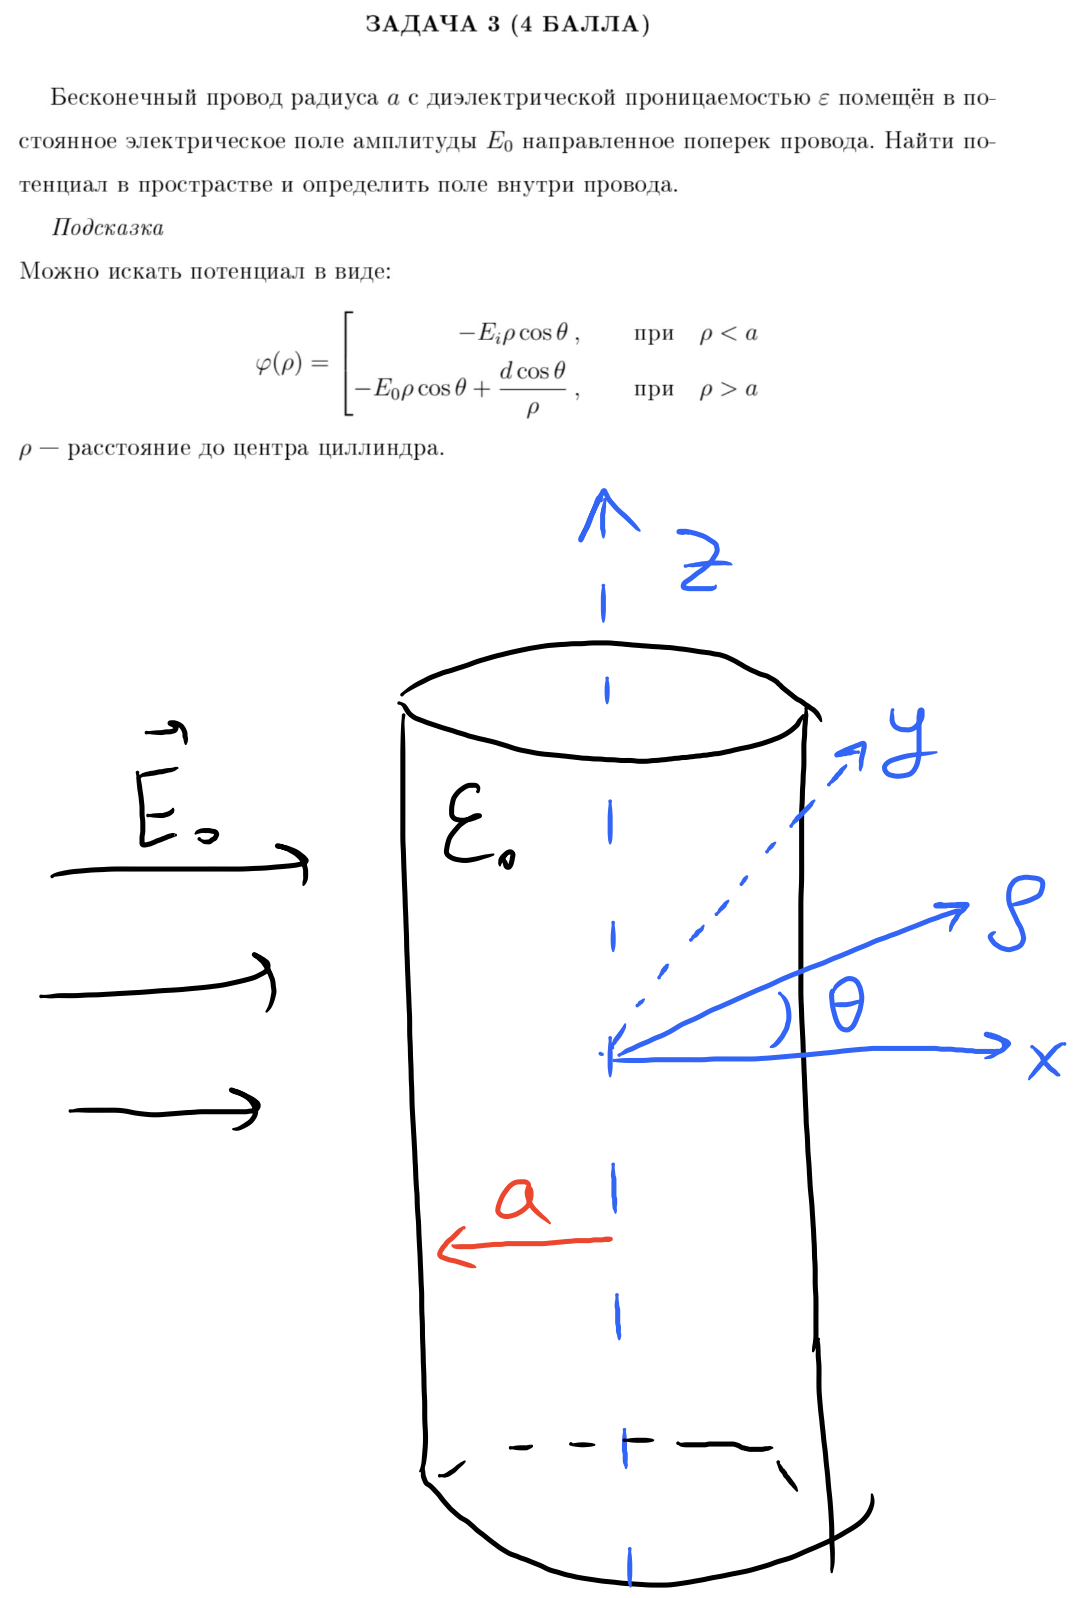
\includegraphics[width=\textwidth]{photo.png}
%\begin{center}
%\underline{Рисунок 1}:
%\end{center}
\par Решение:
\[
    \Delta \overrightarrow{B} = \frac{4\pi e^2 n}{c^2 m} \overrightarrow{B} \Rightarrow \Delta \overrightarrow{B} = \frac{\overrightarrow{B}}{\Lambda^2}
\]
\par Введем цилиндрические координаты
\par Лапласиан:
\[
    \Delta = \frac{1}{r} \frac{\partial}{\partial r} \left( r \frac{\partial}{\partial r} \right) + \frac{1}{r^2} \frac{\partial^2}{\partial \varphi^2} + \frac{\partial^2}{\partial z^2}
\]
\par При $r > r_0$
\[
    \Delta \overrightarrow{B} = 0  \Rightarrow \overrightarrow{B}(r) = \overrightarrow{B_0}
\]
\par При $r \leqslant r_0$
\[
   \Delta \overrightarrow{B} = \frac{\overrightarrow{B}}{\Lambda^2}
\]
\par
\[
    \frac{1}{r} \frac{\partial}{\partial r} \left( r \frac{\partial \overrightarrow{B}}{\partial r} \right) = \frac{\overrightarrow{B}}{\Lambda^2}
\]
\par
\[
    \frac{\partial^2 \overrightarrow{B}}{\partial r^2} + \frac{1}{r} \frac{\partial \overrightarrow{B}}{\partial r} - \frac{\overrightarrow{B}}{\Lambda^2} = 0
\]
\par Замена: $r = \Lambda \rho$
\[
   \frac{\partial^2 \overrightarrow{B}}{\partial \rho^2} + \frac{1}{\rho} \frac{\partial \overrightarrow{B}}{\partial \rho} - \overrightarrow{B} = 0
\]
\par
\[
    \overrightarrow{B} = B_z \overrightarrow{e_z}
\]
\par
\[
    \frac{\partial^2 B_z}{\partial \rho^2} + \frac{1}{\rho} \frac{\partial B_z}{\partial \rho} - B_z = 0
\]
\par Будем искать решение уравнения в виде:
\[
   B_z(\rho) = C \cdot I_0(\rho) + D \cdot K_0(\rho)
\]
\par Функция $K_0(\rho) \rightarrow +\infty$ при $\rho \rightarrow 0$
\par $B_z(\rho)$ - ограничена при $\rho = 0 \Rightarrow D = 0$
\[
    \Rightarrow B_z(\rho) = C \cdot I_0(\rho)
\]
\[
    \Rightarrow B_z(r) = C \cdot I_0(r/\Lambda)
\]
\par Непрерывность тангенсеальной компоненты поля:
\[
    B_{\tau}|_{r_0 + 0} - B_{\tau}|_{r_0 - 0} = 0
\]
\[
    B_0 = C \cdot I_0(r_0/\Lambda) \Rightarrow C = \frac{B_0}{I_0(r_0/\Lambda)}
\]
\par Получаем:
\[
    \overrightarrow{B}(r) = \frac{B_0 \overrightarrow{e_z}}{I_0(r_0/\Lambda)} I_0(r/\Lambda); \text{ при } r \leqslant r_0
\]
\par
\[
    \overrightarrow{B}(r) = B_0 \overrightarrow{e_z}; \text{ при } r > r_0
\]
\par Найдем $\vec{j}$
\[
    rot \overrightarrow{B} = \frac{4\pi}{c} \vec{j}
\]
\begin{multline*}
    \vec{j} = \frac{c}{4\pi} \left( \frac{1}{r} \frac{\partial B_z}{\partial \varphi} - \frac{\partial B_\varphi}{\partial z} \right) \overrightarrow{e_r} + \left( \frac{\partial B_r}{\partial z} - \frac{\partial B_z}{\partial r} \right) \overrightarrow{e_\varphi} + \frac{1}{r} \left( \frac{\partial(rB_\varphi)}{\partial r} - \frac{\partial B_r}{\partial \varphi} \right) \overrightarrow{e_z} =
    \end{multline*}
\[
    = -\frac{c}{4\pi} \frac{\partial B_z}{\partial r} \overrightarrow{e_\varphi} = -\frac{c}{4\pi} \frac{B_0 \overrightarrow{e_\varphi}}{I_0(r_0/\Lambda)} \frac{1}{\Lambda} I'_0(r/\Lambda)
\]
\par Используя рекуррентные соотношения, получаем:
\[
   \vec{j} = -\frac{c}{8\pi} \frac{B_0 \overrightarrow{e_\varphi}}{I_0(r_0/\Lambda)} \frac{1}{\Lambda} \left( I_{-1}(r/\Lambda) + I_{+1}(r/\Lambda) \right) = -\frac{c}{4\pi} \frac{B_0 \overrightarrow{e_\varphi}}{I_0(r_0/\Lambda)} \frac{1}{\Lambda} I_{+1}(r/\Lambda)
\]
\par Ответ:
\[
    \overrightarrow{B}(r) = \frac{B_0 \overrightarrow{e_z}}{I_0(r_0/\Lambda)} I_0(r/\Lambda); \text{ при } r \leqslant r_0
\]
\par
\[
    \overrightarrow{B}(r) = B_0 \overrightarrow{e_z}; \text{ при } r > r_0
\]
\par
\[
   \vec{j}(r) = -\frac{c}{4\pi} \frac{B_0 \overrightarrow{e_\varphi}}{I_0(r_0/\Lambda)} \frac{1}{\Lambda} I_{+1}(r/\Lambda)
\]
\end{large}
\end{document}
